\section{Databases and Sets}
This section deals with some definitions and how to formulate SQL Queries
\subsection{Definitions}
\paragraph{Relations}
\begin{itemize}
	\item Domain (D): An arbitrary (non-null) set of atomic values
	\item Attribute Name (A): A symbol with an associate domain
	\item Relational Schema (R): A finite set of attribute names
	\item Tuple (t): a mapping from the attributes of a relational schema to the union of their domains
	\item Relation (r): A finite set of tuples of relational schema
	\item Degree: Number of attributes [columns in an SQL table]
	\item Cardinality: Number of tuples [rows in an SQL table]
\end{itemize}
\paragraph{Keys}
\begin{itemize}
	\item Superkey: a set of attributes that can \textit{always} be used to differentiate one tuple from another
	\item Key - a minimal superkey
	\item Concatenated Key -  a key with more than one attribute
	\item Candidate Key - any key
	\item \textbf{Primary Key} - one of the candidate keys used to reference from other relations
	\item \textbf{Foreign Key} - an attribute of the relation which is a key for another relation
\end{itemize}
\paragraph{Data Types}
\begin{itemize}
	\item BOOLEAN: TRUE, FALSE, or NULL
	\item Strings: 
	\begin{itemize}
		\item CHAR(length)
		\item CHARACTER(length)
		\item VARCHAR
		\item TEXT
	\end{itemize}
	\item INTEGER
	\item REAL: A floating point
	\item Arbitrary Precision:
		\begin{itemize}
			\item NUMERIC
			\item DECIMAL
			\item MONEY
		\end{itemize}
	\item Date and Time
		\begin{itemize}
			\item TIMESTAMP
			\item DATE
			\item TIME
		\end{itemize}
\end{itemize}
\paragraph{Constraints}
\begin{itemize}
	\item DOMAIN: The domain/type of the attributes; eg INTEGER, VARCHAR
	\item NOT NULL: Ensures the column will not have a null value
	\item UNIQUE: Ensures uniqueness
	\item PRIMARY KEY: Not-null, unique column used as a primary identifier of a row
	\item FOREIGN KEY: Unique identifier to a row from another table
	\item CHECK(condition): Ensures all values in the column meet the defined condition (eg. cost $>$ 10)
	\item DEFAULT(default): Sets the value to the given value if no other value is specified on creation
\end{itemize}
\paragraph{Foreign Key Syntax}
\begin{itemize}
	\item ON DELETE (action): Does the specified action when the key or referenced table is deleted
	\item ON UPDATE (action): Does the specified action when the key or referenced table is updated
	\item NO ACTION: Action - Does nothing
	\item RESTRICT: Action - will not allow user to delete/update the key/referenced table
	\item CASCADE: Action - cascades the change on the original to the value found in the foreign table
	\item SET NULL: Action - sets the value to null in the foreign table
	\item SET DEFAULT: Action - sets the value to default in the foreign table
\end{itemize}

\subsection{SQL Statements}
\paragraph{CREATE}
\begin{verbatim}
CREATE TABLE tableName (
    attributeName TYPE CONTRAINTS,
    attributeName2 TYPE CONTRAINTS,
    exampleID TYPE CONSTRAINTS,
    exampleID2 TYPE CONSTRAINTS,

    PRIMARY KEY (exampleID),
    FOREIGN KEY (exampleID2) REFERENCES  otherTable(id)
        ON UPDATE action
        ON DELETE action;
)
\end{verbatim}

\paragraph{INSERT}
\begin{verbatim}
    INSERT INTO tableName VALUES  (valueA, valueB, valueC, ...);

    INSERT INTO tableName(attributeA, attributeB, attributeC) 
        VALUES  (valueA, valueB, valueC);
\end{verbatim}

\paragraph{UPDATE}
\begin{verbatim}
    UPDATE tableName SET attributeA = valueA WHERE id = valueID;
\end{verbatim}

\paragraph{DELETE}
\begin{verbatim}
    DELETE FROM tableName WHERE attributeA = valueA;
\end{verbatim}

\paragraph{SELECT}
\begin{verbatim}
    SELECT * AS resultTableName FROM tableName WHERE condition;
\end{verbatim}
\paragraph{Selections}
\begin{itemize}
	\item *: Returns every attribute
	\item attributeName1, attributeName2, ...: Returns the requested attributes only
	\item tableName1.attributeName, tableName2.attributeName: Returns values from multiple tables
\end{itemize}
\paragraph{ORDER BY}
\begin{verbatim}
    SELECT * FROM tableName ORDER BY column1, column2, ... ASC|DESC;
\end{verbatim}
Orders the result table in the defined ordered. Can be in ascending (ASC) or descending (DESC) order. Usually defaults to ASC.
\paragraph{DISTINCT}
\begin{verbatim}
    SELECT DISTINCT column1 FROM tableName;
\end{verbatim}
The SELECT DISTINCT statement is used to return only distinct (different) values. Inside a table, a column often contains many duplicate values; and sometimes you only want to list the different (distinct) values.
\paragraph{WHERE}
\begin{verbatim}
    SELECT * AS resultTableName FROM tableName WHERE condition AND|NOT condition;
\end{verbatim}
Where uses a boolean condition and returns a resultTable where each row matches the given condition (or conditions)
\paragraph{LIKE}
\begin{verbatim}
    SELECT * AS resultTableName FROM tableName WHERE condition LIKE pattern;
\end{verbatim}
Like is used in the where condition and allows for checking of a specified pattern. There are two wildcard characters you can use in LIKE.
\begin{itemize}
	\item \% - Represents zero, one, or multiple characters (eg. \%a\% matches with Faisal)
	\item \_ - Represents a single character (eg. a\_ does not match with Rajhi)
\end{itemize}
\paragraph{FUNCTIONS}
\begin{verbatim}
    SELECT FUNCTION(column) AS resultTableName FROM tableName;
\end{verbatim}
Some predefined functions:
\begin{itemize}
	\item COUNT(): Returns the number of rows in the supposed resultant table
	\item SUM(): Returns the sum of a numerical column
	\item AVG(): SUM()/COUNT()
\end{itemize}
\paragraph{JOIN}
\begin{verbatim}
    SELECT a.column, b.column 
    FROM tableName1 a 
    (INNER|LEFT|RIGHT|FULL OUTER) JOIN tableName2 b 
    ON a.column = b.column;
\end{verbatim}
A JOIN clause is used to combine rows from two or more tables, based on a related column between them. There are a few types of joins. Joins also removed duplicates, a sort of built in DISTINCT
\begin{itemize}
	\item INNER: Returns records that have matching values in both tables
	\item LEFT: Return all records from the left table and the matched record from the right table
	\item RIGHT: Return all records form the right table and the matched record from the left table
	\item FULL OUTER: Return all records matched from either table
\end{itemize}
\paragraph{UNION}
\begin{verbatim}
    SELECT * AS resultTableName1 FROM tableName1
    UNION (ALL|)
    SELECT * AS resultTableName2 FROM tableName2;
\end{verbatim}
Union combines the query from multiple SELECT statements. It automatically removes duplicates, to maintain duplicates, use UNION ALL.
\paragraph{SUBQUERY}
\begin{verbatim}
    SELECT * AS resultTableName1 
        FROM (
            SELECT * FROM tableName2
        ) ;
\end{verbatim}
Subqueries run a query on a result table instead of a table/set of tables from the database. Just us normal parenthesis ().
\paragraph{GROUP BY}
\begin{verbatim}
    SELECT COUNT(column1), column2
    FROM tableName
    GROUP BY column2
    ORDER BY COUNT(column1) DESC;
\end{verbatim}
Usually used with functions, groups resultant values with one or more columns. For example, counting how many times each country appears in a table; using group by will place the count next to its respective country.
\paragraph{HAVING}
\begin{verbatim}
    SELECT COUNT(column1), column2
    FROM tableName
    GROUP BY column2
    HAVING condition //eg HAVING COUNT(column1) > 3
    ORDER BY COUNT(column1) DESC;
\end{verbatim}
HAVING exists because SQL people realized WHERE didn't work with functions. Use this with count, sum and all that jazz.
\section{JDBC}
We won't be covering details regarding JDBC and how to use it (such as using Connection objects or how to insert password) since that is more programming and should be covered already.
\subsection{Statements}
There are two types of statement objects; Statement and PreparedStatement. Statements are simply strings that get converted to an SQL Query, whereas PreparedStatements are a little more modular. PreparedStatements are a generic sort of strings, with a variable, usually denoted by ?, that can be replaced and dynamically altered. There a few benefits to using PreparedStatements;
\begin{enumerate}
	\item Reusable and dynamic, so its faster
	\item Seperates logic of query and parameters, so its clearer to code for
	\item No need to convert parameters to Strings, so its faster and uses less bandwidth
	\item More generic, so its type safe
	\item Protects against SQL injection (mostly), so its more secure
\end{enumerate}
SQLInjection is a sort of security hax that injects SQL code as an input from the user and returns undesired results. Sanitizing results can help against such security risks, but its much easier to at the very least use preparedStatements for most queries.

Note; concurrency and race conditions can also cause issues for databases that need to be accurate, such as banks. Databases can handle these things via "transactions", but also these issues can arise from code. Each concurrency issue needs to be handled on its own. A race condition needs synchronicity, but it could cause large queues and slow downs. The solution to these issues is on a system to system basis, but they should be noted.
\section{ER Diagrams}
Entity Relation (ER) Diagrams are graphical representations of tables, and are a database design practice used to, well, design a database. ER Diagrams are easily converted to SQL Create statements and tables. Shapes in an ER diagram mean different things.
\begin{itemize}
	\item DIAMOND: A relation set (A shop needs customers and an inventory; the shop is a relation set)
	\item RECTANGLE: An entity set (The customers and inventory are entities)
	\item OVAL: An attribute (The customers have names; these are attributes)
\end{itemize}
We also use some special marks or labels that can different meanings.
\begin{itemize}
	\item Line: Defines a connection/relationship between two things
	\item Cardinality: Number placed next to the shape on a line. For example, [Students] 3 -> 1 [Course] means that Each Student has only 1 course, and each course has 3 Students.
	\item Underline: Underlining an attribute represents that at is a Primary Key
	\item Double Outline: An entity with a double outline is a weak entity; one that depends entirely on another.
\end{itemize}
Consider this example from the lecture. Every rental must record the date and time at which the rental started and finished, the details of the driver and the details of the car rented. Each car has its registration number recorded, the date it was purchased and a record of all maintenance work undertaken. For a driver, the company needs to have their name, driver’s licence number, address and at least one telephone number. \newline
\begin{figure}[!htb]
	\center{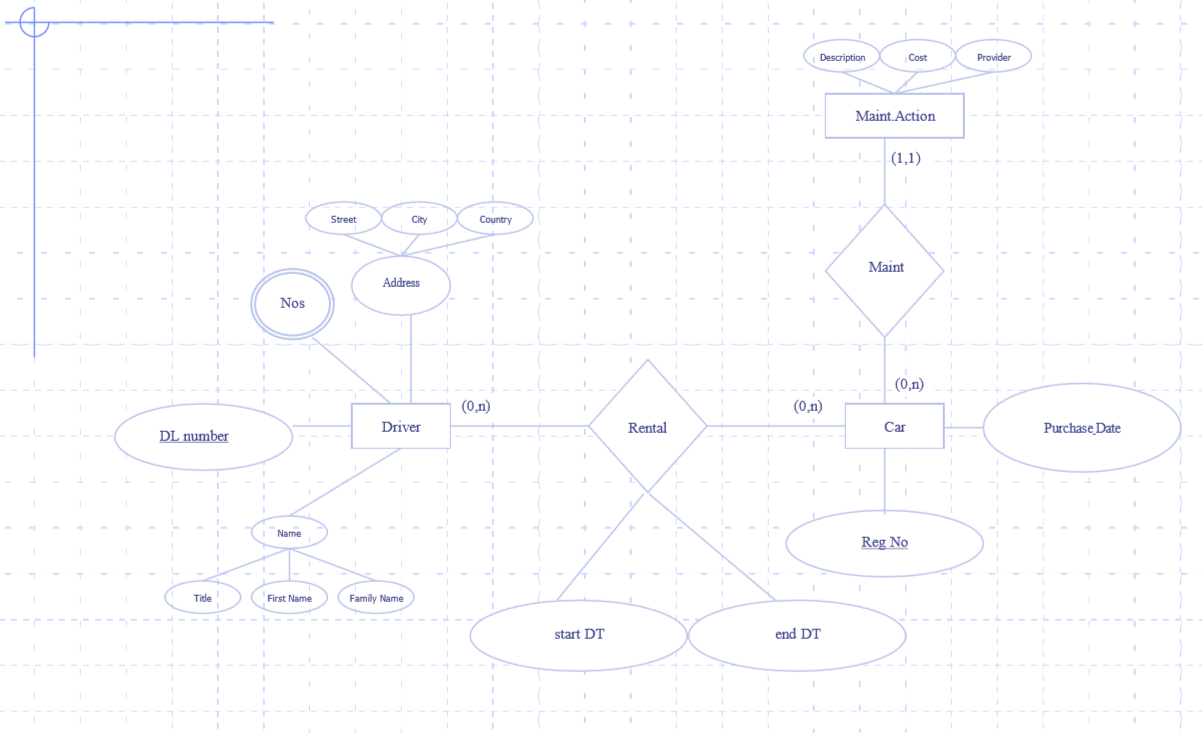
\includegraphics[width=18cm]
		{database/er}}
	\caption{\label{fig:er} ER Diagram Example Solution}
\end{figure}


NOTE: Your ER diagram does not have to look like this to be correct, there can be multiple variations.